\newpage
\section{Discontinuous Galerkin Method}

The Discontinuous Galerkin Method is a method of resolving differential equations through a mesh. It is similar to the Finite Element Method and the Finite Volume Method. This section is for the reader with a beginner's understanding of the Finite Element Method.

\subsection{Basic Overview}


\begin{figure}[ht]
\centering
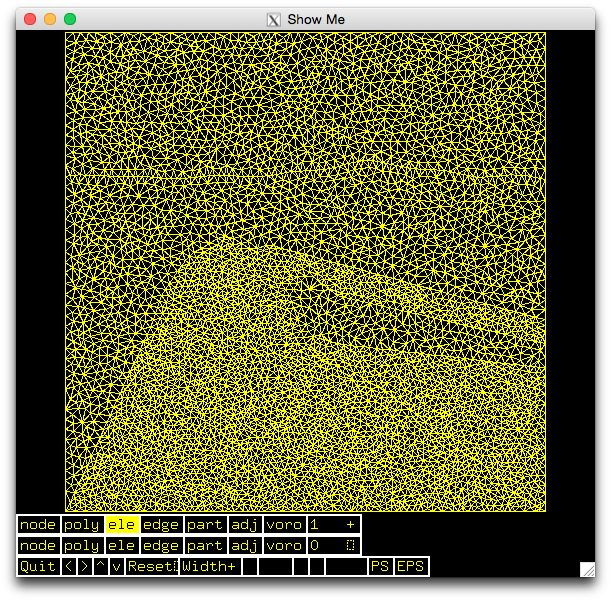
\includegraphics[width=0.7\textwidth]{Images/Example-Mesh.png}
\caption{Example Mesh used to cover example data}
\label{fig:couches5-mesh}
\end{figure}

"Solving differential equations" (such as the acoustic wave equation) is a term that is commonly thrown around without much attention to the essential components in numerical analysis. For the common case, it means: \textbf{given a domain} (for example $[0,10]$ in one dimension or the unit sphere in three dimensions), we \textbf{take a mesh} (set of segments, triangles, tetrahedrons, etc) that covers the domain, and find the values of the variable we are solving for at \textbf{certain moments in time} and at \textbf{certain points in the domain} that are determined by the mesh.

The Discontinuous Galerkin Method is a method to "solve differential equations". It can be considered a combination of Finite Element Methods (Continuous Galerkin) and Finite Volume Methods. In other words, Discontinuous Galerkin methods are finite element methods that use discontinuous basis functions, thus acquiring more robustness for discontinuous processes. Because the base function polynomials are discontinuous and do not extend over a large stencil,the  Discontinuous Galerkin Method is easily parallelized, and the Mass Matrix is able to be inverted by blocks. Like the Finite Volume Methods, Discontinuous Galerkin methods calculate surface integrals and fluxes of discontinuous terms.

\subsection{Basis Functions}

In Discontinuous Galerkin Methods, we can raise the accuracy of our solution by increasing the order of the polynomials that approximate it. 

The way we represent our solution to the differential equation, is a group of polynomials for each element in the mesh; each polynomial takes a value of $1$ at a certain point called a node, and $0$ at all the other nodes defined in the element. Each base function is discontinuous in that it can take nonzero values inside its own element, but takes the value $0$ on other elements. This is the reason the method is called Discontinuous Galerkin and also the fundamental reason it is easily parallelizable. We can thus define the solution as the linear combination of those functions:

$$u(x,t) = \sum\limits_{i=0}^n c_i(t)\phi_i(x)$$ 
where $c_i(t)$ is merely a time-dependent coefficient and $\phi_i(x)$ is the space-dependent base function defined solely on its corresponding element.


But an important observation that helps us significantly speed up the computation is realizing that we can perform all our integrals on a simple reference element, and then map it onto the actual element. Refer to Figure ~\ref{fig:Reference-Elements} for the visual definition of the reference element in 2 and 3 dimensions as well as the transformation mapping. Here we let the use of the hat in $\hat{F}$ represent the reference element, and the lack of use represent the actual element.


\begin{figure}[ht]
	\centering
	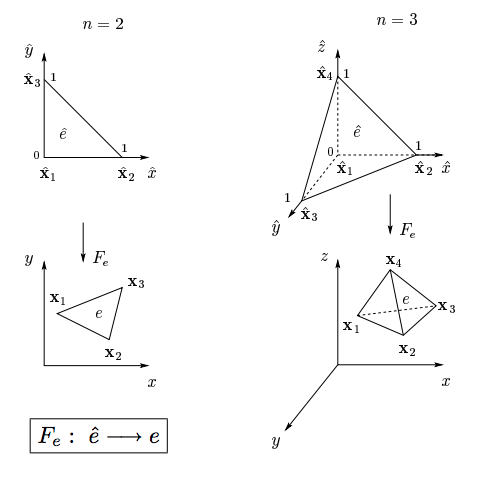
\includegraphics[width=0.7\textwidth]{Images/Reference-Elements.png}
	\caption{Reference Elements transformed to the actual Elements}
	\label{fig:Reference-Elements}
\end{figure}


Given an order $p$, the specific nodes on the reference element are defined as:

$$(\hat{x_i}, \hat{y_j}, \hat{z_k}) = \left( \frac{i}{p}, \frac{j}{p}, \frac{k}{p} \right) \text{ for each } (i,j,k) \in \mathbb{N}^3 \mid i + j + k \leq p$$ 

In order to calculate the base functions for the arbitrary order $p$, we can use linear algebra. Namely, we wish to find the base function polynomials of the form:

$$\sum\limits_{i+j+k \leq p} C_{i,j,k} x^i y^j z^k = \sum\limits_{j=1}^n C_j m_j(x)$$
where we have $n$ nodes, $n$ polynomials, and $n$ monomials per polynomial. 

Because the $i$'th polynomial takes a value of $1$ at the $i$'th node and $0$ at all the others, we can represent this relationship with a matrix equation, where the vector on the right is the $i$'th unit vector:

$$\begin{bmatrix}
m_1(x_1) & m_2(x_1) & m_3(x_1) & \ldots \\
m_1(x_2) & m_2(x_2) & m_3(x_2) & \ldots \\
m_1(x_3) & m_2(x_3) & m_3(x_3) & \ldots \\
\ldots & \ldots & \ldots & \ldots 
\end{bmatrix} 
\begin{bmatrix}
C_1 \\
C_2 \\
C_3 \\
\ldots
\end{bmatrix}
= \begin{bmatrix}
0 \\
\ldots \\
1 \\
\ldots
\end{bmatrix} $$

We can find the polynomial by computing the values of $C_j$,
and summing their product with their corresponding monomials. For simplicity, represent the equation as $V \boldsymbol{C} = \boldsymbol{I}$. By multiplying both sides by $V^{-1}$, we have that $\boldsymbol{C}$ is equal to the $i$'th column of of $V^{-1}$. Thus, we have our $i$'th base function polynomial.

\subsection{Decomposing u(x,t)}

We can decompose 

\subsection{Random Thoughts to be organized later}

We can decompose u(x,t) into discontinuous space-dependent parts and time dependent parts. We let $u(x,t) = c_1(t) \phi_1(x) + c_2(t) \phi_2(x) + \ldots + c_n(t) \phi_n(x)$. 

With this method, we can then transform the equations into a linear matrix form. For example, take the term $\int_K \frac{\partial^2 u(x,t)}{\partial t^2} v(x,t) dV$.

$$\int_K \frac{\partial^2 u(x,t)}{\partial t^2} v(x,t) dV$$

We want the equalities to be satisfied for any $v(x,t)$ in our function space, so we just need to make sure that the equalities are satisfied for $v(x,t) = \phi_i(x)$ for all $i$. We can do this by using vector and matrix operations to represent multiple equations.


$$\begin{bmatrix}
\int u(x,t) \phi_1 dV \\
\int u(x,t) \phi_2 dV \\
\ldots \\
\int u(x,t) \phi_n dV
\end{bmatrix}$$

$$= \begin{bmatrix}
\int \frac{\partial^2 c_1(t)}{\partial t^2} \phi_1 \phi_1 dV \\
\int \frac{\partial^2 c_2(t)}{\partial t^2} \phi_1 \phi_2 dV \\
\ldots \\
\int \frac{\partial^2 c_n(t)}{\partial t^2} \phi_1 \phi_n dV
\end{bmatrix}$$

$$= \begin{bmatrix}
    \int \phi_1 \phi_1 dV & \int \phi_1 \phi_2 dV & \int \phi_1 \phi_3 dV & \ldots \\
    \int \phi_2 \phi_1 dV & \int \phi_2 \phi_2 dV & \int \phi_2 \phi_3 dV & \ldots \\
    \int \phi_3 \phi_1 dV & \int \phi_3 \phi_2 dV & \int \phi_3 \phi_3 dV & \ldots \\
    \ldots & \ldots & \ldots & \ldots 
\end{bmatrix} 
\frac{\partial^2}{\partial t^2} 
\begin{bmatrix}
    c_1(t) \\
    c_2(t) \\
    c_3(t) \\
    \ldots
\end{bmatrix} $$

$$= M \frac{\partial^2}{\partial t^2} U_h$$
where $M$ is the Mass matrix and $U_h$ is the vector of coefficients defining $u(x,t)$


